\chapter{Полносвязные модели}
\label{chap:fully_connected_models}

\begin{supportbox}{Об этой главе}
Стандартное программирование осуществляется путем объединения соответствующих примитивных операций. В этой главе мы покажем, что можем сделать нечто подобное для дифференцируемых моделей, составляя последовательность так называемых \textit{полносвязных слоев}. По историческим причинам эти модели также известны как многослойные перцептроны (МЛП). МЛП строятся путем чередования линейных блоков (аналогично Главе \ref{chap:linear_models}) с нелинейными функциями, иногда называемыми \textit{функциями активации}.
\end{supportbox}

\section{Ограничения линейных моделей}

Линейные модели принципиально ограничены, в том смысле, что по определению они не могут моделировать нелинейные зависимости между признаками. В качестве примера рассмотрим два входных вектора $\mathbf{x}$ и $\mathbf{x}^\prime$, которые идентичны, за исключением одного признака с индексом $j$:
%
$$
x_i^\prime=\begin{cases} x_i & \text{ если } i \neq j \\ 2x_i & \text{ иначе } \end{cases}
$$
%
Например, это могут быть два клиента банка, которые идентичны во всех отношениях, кроме их дохода, причем у $\mathbf{x}^\prime$ доход вдвое больше, чем у $\mathbf{x}$. Если $f$ — линейная модель (без смещения), мы имеем:

\vspace{1em}
\begin{equation*}
f(\mathbf{x}^\prime) = \eqnmarkbox[drawred]{node}{f(\mathbf{x})} + \eqnmarkbox[drawblue]{node2}{w_jx_j}
\end{equation*}
\annotate[yshift=1em]{above,left}{node}{Исходный выход}
\annotate[yshift=1em]{above,right}{node2}{Изменение, вызванное $x_j^\prime = 2x_j$}

Следовательно, единственным следствием изменения входа является небольшое линейное изменение выхода, продиктованное $w_j$. Предположим, мы оцениваем пользователей, мы можем захотеть смоделировать такие зависимости, как «\textit{доход 1500 является низким, за исключением случаев, когда возраст < 30}».\footnote{В любом случае, вам, вероятно, не следует заниматься кредитным скорингом с помощью машинного обучения.} Очевидно, что это невозможно сделать с помощью линейной модели из-за приведенного выше анализа. 

Прототипическим примером этого является набор данных XOR, двузначный набор данных, где каждый признак может принимать значения только в $\left\{0, 1\right\}$. Следовательно, весь набор данных задается всего 4 возможностями:
%
$$
f([0,0])=0 \;,\; f([0,1])=1\;,\;f([1,0])=1\;,\;f([1,1])=0
$$
%
где выход положителен, когда \textit{только один} из двух входов положителен. Несмотря на свою простоту, это также \textbf{нелинейно разделимо} и не может быть решено со 100\% точностью линейной моделью - см. Рисунок \ref{fig:xor} для визуализации.

\begin{SCfigure}
    \centering
    \hspace{1em}\includegraphics[width=0.5\textwidth]{images/XOR.pdf}
    \caption{Иллюстрация набора данных XOR: зеленые квадраты — это значения одного класса, красные круги — значения другого класса. Никакая линейная модель не может разделить их идеально (поместив все квадраты по одну сторону, а все круги — по другую сторону от границы решения). Мы говорим, что набор данных не является \textbf{линейно разделимым}.}
    \label{fig:xor}
\end{SCfigure}


\section{Композиция и скрытые слои}

\addclock Мощная идея в программировании — это декомпозиция, т.е. рекурсивное разбиение задачи на составные части, пока каждая часть не сможет быть выражена в простых, управляемых операциях. Нечто подобное можно достичь и в нашем случае, представив, что наша модель $f$ на самом деле является композицией двух обучаемых операций:

$$
f(\mathbf{x})=(f_2 \circ f_1)(\mathbf{x})
$$

где $f_2 \circ f_1$ — это композиция двух функций: $(f_2 \circ f_1)(\mathbf{x}) = f_2(f_1(\mathbf{x}))$, и мы предполагаем, что каждая функция инстанцирует свой собственный набор обучаемых параметров. Мы можем продолжать подразделять вычисления:

$$
f(\mathbf{x})=(f_l\circ f_{l-1}\circ \cdots\circ f_2\circ f_1)(\mathbf{x})
$$

где у нас теперь в общей сложности $l$ функций, которые компонуются. Обратите внимание, что пока каждая $f_i$ не изменяет «тип» своих входных данных, мы можем связывать вместе столько этих преобразований, сколько захотим, и каждое из них будет добавлять свой собственный набор обучаемых параметров. 

Например, в нашем случае вход $\mathbf{x}$ — это вектор, следовательно, любая операция «вектор-в-вектор» (например, умножение матрицы $f_i(\mathbf{x}) = \mathbf{W}\mathbf{x})$ может быть объединена вместе бесконечное количество раз. Однако следует соблюдать некоторую осторожность. Предположим, мы связываем вместе две разные линейные проекции:
%
\begin{gather}
\mathbf{h} = f_1(\mathbf{x}) = \mathbf{W}_1\mathbf{x} +\mathbf{b}_1 \\y=f_2(\mathbf{h})=\mathbf{w}^\top_2\mathbf{h} + b_2
\end{gather}

Легко показать, что две проекции «схлопываются» в одну:

$$
y = \underbrace{(\mathbf{w}^\top_2\mathbf{W}_1)}_{\triangleq\;\mathbf{A}}\mathbf{x} + \underbrace{(\mathbf{w}_2^\top\mathbf{b}_1 + b_2)}_{\triangleq \;\mathbf{c}} = \mathbf{A}\mathbf{x}+\mathbf{c}
$$
%
Идея \textbf{полносвязных} (FC) моделей, также известных по историческим причинам как \textbf{многослойные перцептроны} (MLP), заключается во вставке простой поэлементной нелинейности $\phi : \mathbb{R} \rightarrow \mathbb{R}$ между проекциями, чтобы избежать схлопывания:

\vspace{0.5em}
\begin{equation}
\mathbf{h} = f_1(\mathbf{x}) = \eqnmarkbox[drawred]{node}{\phi}\left(\mathbf{W}_1\mathbf{x} +\mathbf{b}_1\right)
\label{eq:mlps_single_hidden_layer_1}
\end{equation}%
\annotate[yshift=0.7em]{above,right}{node}{Поэлементная нелинейность}
%
\begin{equation}
y=f_2(\mathbf{h})=\mathbf{w}^\top_2\mathbf{h} + b_2
\label{eq:mlps_single_hidden_layer_2}
\end{equation}

Второй блок может быть линейным, как в \eqref{eq:mlps_single_hidden_layer_2}, или он может быть обернут в другую нелинейность в зависимости от задачи (например, функцию softmax для классификации). Функция $\phi$ может быть любой нелинейностью, например, полиномом, квадратным корнем или функцией сигмоида $\sigma$. Как мы увидим в следующей главе, ее выбор оказывает сильное влияние на градиенты модели и, следовательно, на оптимизацию, и задача состоит в том, чтобы выбрать $\phi$, которая является «достаточно нелинейной», чтобы предотвратить схлопывание, оставаясь при этом как можно ближе к тождественной функции в своей производной. Хорошим выбором по умолчанию является так называемый \textbf{выпрямленный линейный блок} (ReLU). 

\begin{definition}[Выпрямленный линейный блок] \addbottle
\textbf{Выпрямленный линейный блок} (ReLU) определяется поэлементно как:
%
\begin{equation}
\textnormal{ReLU}(s)=\max(0,s)
\label{eq:relu}
\end{equation}
\end{definition}

Мы еще многое скажем о ReLU в следующей главе. С добавлением $\phi$ мы теперь можем связывать столько преобразований, сколько захотим:

\begin{equation}
y = \mathbf{w}_l^\top\phi\left( \mathbf{W}_{l-1}\left(\phi\left( \mathbf{W}_{l-2}\phi\left(\cdots\right)+\mathbf{b}_{l-2} \right)\right)+\mathbf{b}_{l-1} \right) + b_l
\label{eq:mlps_multiple_hidden_layer}
\end{equation}

В остальной части главы мы сосредоточимся на анализе свойств обучения и аппроксимации этого класса моделей. Но сначала краткое отступление о соглашениях об именах.

\subsection*{О терминологии, используемой в дифференцируемых моделях}

Как мы уже упоминали, нейронные сети имеют долгую историю и большой багаж терминологии, которую мы кратко резюмируем здесь. Каждая $f_i$ называется \textbf{слоем} модели, где $f_l$ — \textbf{выходной слой}, $f_{i}, i=1,\ldots,l-1$ — \textbf{скрытые слои} и, с небольшим злоупотреблением нотацией, $\mathbf{x}$ — \textbf{входной слой}. С этой терминологией мы можем переформулировать определение \textbf{полносвязного слоя} в пакетной форме ниже.

\begin{definition}[Полносвязный слой] \addbottle
Для пакета из $n$ векторов, каждый размером $c$, представленного в виде матрицы $\mathbf{X} \sim (n,c)$, \textbf{полносвязный} (FC) слой определяется как:
%
\begin{equation}
\textnormal{FC}(\mathbf{X}) = \phi\left(\mathbf{X}\mathbf{W} + \mathbf{b}\right)
\label{eq:fully_connected_layer}
\end{equation}
%
Параметрами слоя являются матрица $\mathbf{W} \sim (c^\prime,c)$ и вектор смещения $\mathbf{b} \sim (c^\prime)$, всего $(c^\prime+1)c$ параметров (предполагая, что $\phi$ не имеет параметров). Его гиперпараметрами являются ширина $c^\prime$ и нелинейность $\phi$.
\end{definition}

Выходы $f_i(\mathbf{x})$ называются \textbf{активациями} слоя, где мы иногда можем различать \textbf{преактивацию} и \textbf{постактивацию} (до и после нелинейности). Сама нелинейность $\phi$ может называться \textbf{функцией активации}. Каждый выход $f_i$ называется \textbf{нейроном}. Хотя большая часть этой терминологии устарела, она все еще широко распространена, и мы будем использовать ее при необходимости.

Размер каждого слоя (форма выхода) является гиперпараметром, который может быть выбран пользователем, поскольку он влияет только на форму входа следующего слоя, что известно как \textbf{ширина} слоя. При большом количестве слоев количество гиперпараметров растет линейно, и их выбор становится комбинаторной задачей. Мы вернемся к этому вопросу в Главе \ref{chap:deep_cnns}, когда будем обсуждать проектирование моделей с десятками (или сотнями) слоев.

\begin{mypy}{Слой FC в \eqref{eq:fully_connected_layer}, реализованный как объект в PyTorch. Нам требуется специальный синтаксис для различения обучаемых параметров, таких как $\mathbf{W}$, от других необучаемых тензоров: в PyTorch это достигается путем обертывания тензоров в объект {\footnotesize\mintinline{python}{Parameter}}. В PyTorch также есть своя коллекция слоев в {\footnotesize\mintinline{python}{torch.nn}}, включая слой FC (реализованный как {\footnotesize\mintinline{python}{torch.nn.Linear}}).}{code:fully_connected_layer}
class FullyConnectedLayer(nn.Module):
  def __init__(self, c: int, cprime: int):
    super().__init__()
    # Инициализация параметров
    self.W = nn.Parameter(torch.randn(c, cprime))
    self.b = nn.Parameter(torch.randn(1, cprime))

  def forward(self, x):
    return relu(x @ self.W + self.b)
\end{mypy}

Концепция слоя также широко распространена в распространенных фреймворках. Слой, такой как \eqref{eq:fully_connected_layer}, может быть определен как объект, имеющий две функции: функцию инициализации, которая случайным образом инициализирует все параметры модели на основе выбранных гиперпараметров, и функцию вызова, которая предоставляет выход самого слоя. См. Листинг \ref{code:fully_connected_layer} для примера. Затем модель может быть определена путем объединения экземпляров таких слоев. Например, в PyTorch это можно достичь с помощью объекта {\footnotesize\mintinline{python}{Sequential}}:

\vspace{1em}
{\begin{center}\footnotesize
\begin{minted}{python}
model = nn.Sequential(
    FullyConnectedLayer(3, 5), 
    FullyConnectedLayer(5, 4)
)
\end{minted}
\end{center}}
 
Обратите внимание, что с точки зрения их сигнатуры ввода-вывода нет большой разницы между слоем, определенным в Листинге \ref{code:fully_connected_layer}, и моделью, определенной выше, и мы могли бы эквивалентно использовать \mintinline{python}{model} как слой более крупной модели. Эта композиционность является определяющей характеристикой дифференцируемых моделей.

\subsection{Аппроксимационные свойства МЛП} \addteacup

Обучение МЛП происходит аналогично тому, что мы обсуждали для линейных моделей. Например, для задачи регрессии мы можем минимизировать среднеквадратичную ошибку:
%
$$
\underset{\left\{\mathbf{W}_k, \mathbf{b}_k\right\}_{k=1}^l}{\min} \;\; \frac{1}{n}\sum_{i} \left(y_i - f(\mathbf{x}_i)\right)^2
$$
%
где минимизация теперь выполняется по всем параметрам модели одновременно. В следующей лекции мы увидим общую процедуру вычисления градиентов в этом случае. 

Пока мы отметим, что основное отличие от линейной модели заключается в том, что добавление скрытого слоя делает общую задачу оптимизации невыпуклой, с несколькими локальными оптимумами в зависимости от инициализации модели. Это важный аспект с исторической точки зрения, поскольку альтернативные подходы к обучению с учителем (например, машины опорных векторов \cite{hofmann2008kernel}) предоставляют нелинейные модели, оставаясь при этом выпуклыми. Однако результаты последнего десятилетия показывают, что сильно невыпуклые модели могут достигать значительно хорошей производительности во многих задачах.\footnote{Причина, по которой дифференцируемые модели так хорошо обобщают, является интересным, открытым исследовательским вопросом, к которому мы вернемся в Главе \ref{chap:deep_cnns}. Существующие объяснения варьируются от неявного смещения (стохастического) градиентного спуска \cite{pesme2021implicit} до внутренних свойств самих архитектур \cite{arpit2017closer,teney2024neural}.}

С теоретической точки зрения мы можем спросить, каково значение добавления скрытых слоев, т.е. если линейные модели могут решать только линейно разделимые задачи, то каков класс функций, которые можно аппроксимировать, добавляя скрытые слои? Оказывается, одного скрытого слоя достаточно для \textbf{универсальной аппроксимации}. Основополагающий результат в этом смысле был доказан Г. Цыбенко в 1989 году \cite{cybenko1989approximation}.

\begin{theorem}[Универсальная аппроксимация МЛП \cite{cybenko1989approximation}]
Для непрерывной функции $g: \mathbb{R}^d \rightarrow \mathbb{R}$ мы всегда можем найти модель $f(\mathbf{x})$ вида \eqref{eq:mlps_single_hidden_layer_1}-\eqref{eq:mlps_single_hidden_layer_2} (МЛП с одним скрытым слоем) и сигмоидальными функциями активации, такую, что для любого $\varepsilon > 0$:
%
$$
\lvert f(\mathbf{x}) - g(\mathbf{x})\rvert\le\varepsilon \;,\;\forall \mathbf{x}
$$
%
где результат справедлив для компактной области. Иными словами, МЛП с одним скрытым слоем «плотны» в пространстве непрерывных функций.
\end{theorem}

Красота этой теоремы не должна отвлекать от того факта, что это чисто теоретическая конструкция, которая использует тот факт, что ширина скрытого слоя модели может расти безгранично. Следовательно, для любого $\mathbf{x}$, для которого предыдущее неравенство не выполняется, мы всегда можем добавить новый блок, чтобы уменьшить ошибку аппроксимации (см. Приложение \ref{sec:universal_approximation}). Фактически, можно придумать классы функций, для которых требуемое количество скрытых нейронов растет экспоненциально с числом входных признаков \cite{bengio2009learning}.\footnote{Одна из этих проблем, проблема \textit{четности}, тесно связана с задачей XOR: \url{https://blog.wtf.sg/posts/2023-02-03-the-new-xor-problem/}.}

Многие другие авторы, такие как \cite{hornik1991approximation}, постепенно уточняли этот результат, включая модели с практически любой возможной функцией активации, включая ReLU. Кроме того, универсальная аппроксимация также может быть доказана для моделей с конечной \textit{шириной}, но возможно бесконечной \textit{глубиной} \cite{lu2017expressive}. Отдельное направление исследований изучало аппроксимационные возможности \textit{сверхпараметризованных} моделей, в которых количество параметров превышает количество обучающих данных. В этом случае обучение до глобального оптимума может быть доказано во многих интересных сценариях \cite{du2018gradient,allen2019learning} (неформально, при достаточном количестве параметров модель может достичь минимума потерь на каждом обучающем примере и, следовательно, глобального минимума задачи оптимизации).  См. Приложение \ref{sec:universal_approximation} для одномерной визуализации теоремы Цыбенко.

Аппроксимационные и обучающие возможности дифференцируемых моделей — это огромные области исследований, которым посвящены бесчисленные книги, и мы упомянули здесь лишь некоторые значимые результаты. В остальной части книги мы будем в основном заниматься эффективным проектированием самих моделей, чье поведение может быть более сложным и трудным для контроля (и проектирования), чем предполагают эти теоремы.

\section{Стохастическая оптимизация}

Для оптимизации моделей мы можем выполнять градиентный спуск по соответствующей задаче минимизации эмпирического риска. Однако это может быть труднодостижимо, когда $n$ (размер набора данных) становится очень большим. В следующей главе мы увидим, что вычисление градиента потерь требует времени, линейного по количеству примеров, что становится невозможным или медленным для $n$ порядка $10^4$ и более, особенно для больших моделей (не говоря уже о проблемах с памятью).

К счастью, форма задачи поддается хорошей аппроксимации, где мы используем подмножества данных для вычисления направления спуска. Для этого предположим, что на итерации $t$ градиентного спуска мы выбираем подмножество $\mathcal{B}_t \subset \mathcal{S}_n$ из $r$ точек (где $r \ll n$) из набора данных, которое мы называем \textbf{мини-пакетом}. Мы можем вычислить приближенную потерю, рассматривая только мини-пакет:
%
\begin{equation}
\widetilde{L}_t=\eqnmarkbox[drawred]{node}{\frac{1}{r} {\sum_{(x_i, y_i) \in \mathcal{B}_t}}} l(y_i,f(x_i)) \approx \eqnmarkbox[drawblue]{node2}{\frac{1}{n} {\sum_{(x_i, y_i) \in \mathcal{S}_n}}} l(y_i,f(x_i))
\end{equation}
\annotate[yshift=-1em]{below,left}{node}{Мини-пакет}
\annotate[yshift=-1em]{below,right}{node2}{Полный набор данных}

\vspace{1em}
Если мы предположим, что элементы в мини-пакете выбраны i.i.d. из набора данных, $\widetilde{L}_t$ является аппроксимацией Монте-Карло полной потери, и то же самое справедливо для ее градиента. Однако ее вычислительная сложность растет только с $r$, который может контролироваться пользователем. Грубо говоря, меньшие размеры $r$ мини-пакета приводят к более быстрым итерациям с большей дисперсией градиента, в то время как большие $r$ приводят к более медленным, более точным итерациям. Для больших моделей память, как правило, является самым большим узким местом, и размер мини-пакета $r$ можно выбрать так, чтобы заполнить доступное оборудование на каждой итерации.

\begin{figure}
    \centering
    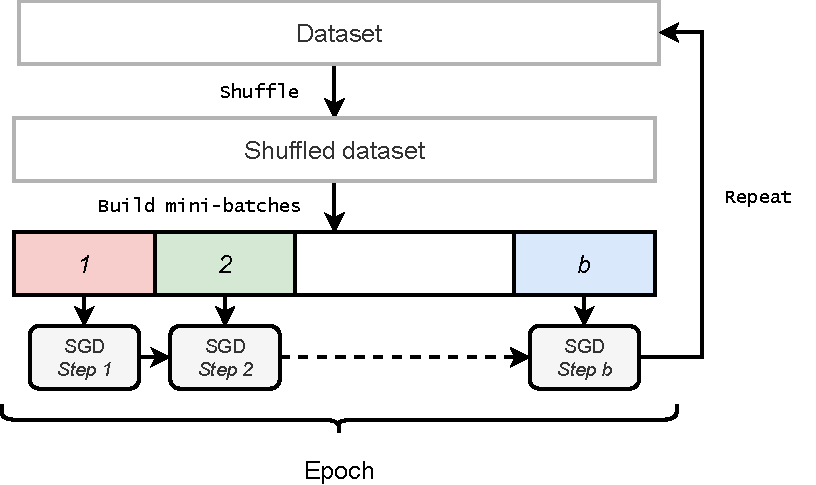
\includegraphics[width=0.7\textwidth]{images/stochastic_optimization.pdf}
    \caption{Построение последовательности мини-пакетов: после перемешивания стохастическая оптимизация начинается с мини-пакета 1, который состоит из первых $r$ элементов набора данных. Она продолжается таким образом до мини-пакета $b$ (где $b = \frac{n}{r}$, предполагая, что размер набора данных идеально делится на $r$). После одной такой \textit{эпохи} обучение продолжается с мини-пакета $b+1$, который состоит из первых $r$ элементов перемешанного набора данных. Вторая эпоха заканчивается на мини-пакете $2b$ и так далее.}
    \label{fig:building_mini_batches}
\end{figure}

Градиентный спуск, применяемый к мини-пакетам данных, является примером \textbf{стохастического градиентного спуска} (SGD). Благодаря описанным выше свойствам, можно доказать, что SGD сходится к минимуму в математическом ожидании, и это предпочтительная стратегия оптимизации при обучении дифференцируемых моделей.

Последняя оставшаяся проблема — как выбирать мини-пакеты. Для больших наборов данных случайная выборка элементов может быть дорогостоящей, особенно если нам нужно перемещать их туда и обратно из памяти GPU. Промежуточное решение, которое поддается более легкой оптимизации, заключается в следующем:

\begin{enumerate}
    \item Начните с перемешивания набора данных.
    \item Затем разделите исходный набор данных на мини-пакеты из $r$ \textit{последовательных} элементов и обрабатывайте каждый из них последовательно. Предполагая набор данных размером $n=rb$, это приводит к $b$ мини-пакетам и, следовательно, к $b$ шагам SGD. Если мы выполняем код на GPU, этот шаг включает отправку мини-пакета в память GPU.
    \item После завершения всех мини-пакетов, построенных таким образом, вернитесь к пункту 1 и повторите.
\end{enumerate}

\begin{mypy}{Построение последовательности мини-пакетов с помощью загрузчика данных PyTorch: все фреймворки предоставляют аналогичные инструменты.}{code:data_loader}
# Набор данных, состоящий из двух тензоров
dataset = torch.utils.data.TensorDataset(
    torch.randn(1000, 3), torch.randn(1000, 1))

# Загрузчик данных обеспечивает перемешивание и разбиение на мини-пакеты
dataloader = torch.utils.data.DataLoader(dataset, 
                shuffle=True, batch_size=32)

for xb, yb in dataloader:
  # Итерация по последовательности мини-пакетов (одна эпоха)
  # xb имеет форму (32, 3), yb имеет форму (32, 1)
\end{mypy}

Один полный цикл этого процесса называется \textbf{эпохой} обучения, и это очень распространенный гиперпараметр для указания (например, для набора данных из $1000$ элементов и мини-пакетов из $20$ элементов, «\textit{обучение в течение 5 эпох}» означает обучение в течение $250$ итераций). Дорогостоящая операция перемешивания выполняется только один раз за эпоху, в то время как между эпохами мини-пакеты могут быть быстро предварительно загружены и оптимизированы фреймворком. Это схематически показано на Рисунке \ref{fig:building_mini_batches}. Большинство фреймворков предоставляют способ организации набора данных в элементы, которые могут быть индивидуально  индексированы, и отдельный интерфейс для построения последовательности мини-пакетов. В PyTorch, например, это делается с помощью интерфейсов {\footnotesize\mintinline{python}{Dataset}} и {\footnotesize\mintinline{python}{DataLoader}} соответственно - см. Листинг \ref{code:data_loader}.


\begin{figure}
    \centering
    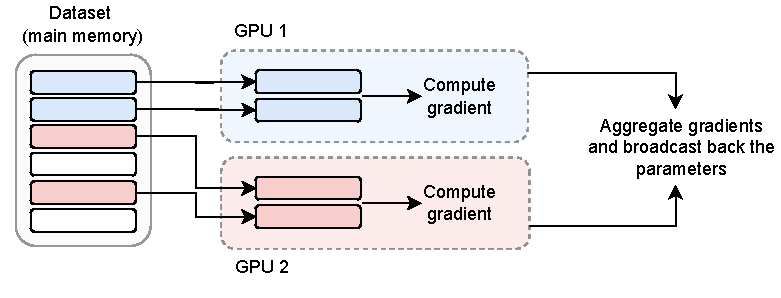
\includegraphics[width=0.75\textwidth]{images/mini_batch.pdf}
    \caption{Простая форма распределенной стохастической оптимизации: мы обрабатываем один мини-пакет на каждой доступной машине или GPU (реплицируя веса на каждой из них) и суммируем или усредняем
    соответствующие градиенты перед трансляцией результата обратно (что допустимо из-за линейности операции градиента). Это требует механизма синхронизации между машинами или GPU.}
    \label{fig:mini_batch}
\end{figure}

Эта схема также поддается простой форме параллелизма между GPU или между машинами. Если мы предположим, что каждая машина достаточно велика, чтобы вместить полную копию параметров модели, мы можем обрабатывать разные мини-пакеты параллельно на машинах, а затем суммировать их локальные вклады для окончательного обновления, которое затем транслируется обратно на каждую машину. Это называется \textbf{параллелизмом данных} в PyTorch,\footnote{\url{https://pytorch.org/tutorials/intermediate/ddp_tutorial.html}} и это визуально показано на Рисунке \ref{fig:mini_batch}. Возможны и более сложные формы параллелизма, такие как \textbf{тензорный параллелизм}, но мы не рассматриваем их в этой книге.


\section{Функции активации}
\label{sec:activation_functions}

Мы завершаем главу кратким обзором выбора функций активации. Как мы уже говорили в предыдущем разделе, теоретически допустима почти любая поэлементная нелинейность. Однако не все варианты имеют хорошую производительность. В качестве примера рассмотрим простую полиномиальную функцию для некоторого заданного пользователем положительного целого числа $p$:
%
$$
\phi(s)=s^p
$$
%
При больших $p$ она будет быстро расти с обеих сторон, накапливаясь по слоям и приводя к моделям, которые трудно обучать и которые имеют численную нестабильность. 

Исторически нейронные сети были введены как приближенные модели биологических нейронов (отсюда и название \textit{искусственные НС}). В этом смысле веса $\mathbf{w}^\top$ в скалярном произведении $\mathbf{w}^\top \mathbf{x}$ были простыми моделями синапсов, смещение $b$ было порогом, и нейрон был «активирован», когда кумулятивная сумма входов превышала порог:
%
$$
s = \mathbf{w}^\top\mathbf{x}-b \;,\; \phi(s)= \mathbb{I}_{s \ge 0}
$$
%
где $\mathbb{I}_{b}$ — это индикаторная функция, которая равна $1$, если $b$ истинно, и $0$ в противном случае. Поскольку эта функция активации недифференцируема, в качестве мягкой аппроксимации можно использовать сигмоиду $\sigma(s)$. Фактически, мы можем определить обобщенную сигмоидальную функцию с настраиваемым наклоном $a$ как $\sigma_a(s) = \sigma(as)$, и мы имеем:
%
$$
\lim_{a \rightarrow \infty}\sigma_a(s)=\mathbb{I}_{s \ge 0}
$$
%
Другим распространенным вариантом был гиперболический тангенс, который является масштабированной версией сигмоиды в $[-1,+1]$:
%
$$
\tanh(s)=2\sigma(s)-1
$$
%
Современные нейронные сети, популяризированные AlexNet в 2012 году \cite{krizhevsky2012imagenet}, вместо этого использовали функцию ReLU в \eqref{eq:relu}. Относительные преимущества ReLU по сравнению с сигмоидоподобными функциями будут обсуждаться в следующей главе. Здесь мы отметим, что ReLU имеют несколько контринтуитивных свойств. Например, у них есть точка недифференцируемости в $0$, и они имеют большую разреженность выхода, поскольку все отрицательные входы устанавливаются в $0$. Это второе свойство может привести к так называемым «мертвым нейронам», когда определенные блоки имеют постоянный выход $0$ для всех входов. Это можно решить с помощью простого варианта ReLU, известного как \textbf{Leaky ReLU}:
%
\begin{equation}
\text{LeakyReLU}(s) = \begin{cases} s & \text{ если } s \ge 0 \\ \alpha s & \text{ иначе } \end{cases} 
\label{eq:leaky_relu}
\end{equation}
%
для очень малого $\alpha$, например, $\alpha = 0.01$. Мы также можем обучать разное $\alpha$ для каждого блока (поскольку функция дифференцируема по отношению к $\alpha$). В этом случае мы называем ФА \textbf{параметрической ReLU} (PReLU) \cite{he2015delving}. Обучаемые функции активации, в общем, являются простым способом добавить небольшое количество гибкости с незначительным количеством параметров — в случае PReLU, один на нейрон.

Также доступны полностью дифференцируемые варианты ReLU, такие как \textbf{softplus}:
%
\begin{equation}
\text{softplus}(s)=\log(1+\exp(s))
\label{eq:softplus}
\end{equation}
%
Softplus не проходит через начало координат и всегда больше $0$. Другой вариант, \textbf{экспоненциальный линейный блок} (ELU), сохраняет прохождение через начало координат, переключая нижнюю границу на $-1$:
%
\begin{equation}
\text{ELU}(s)=\begin{cases} s & \text{ если } s \ge 0 \\ \exp(s)-1 & \text{ иначе } \end{cases}
\label{eq:elu}
\end{equation}
%
Еще один класс вариантов можно определить, заметив сходство ReLU с индикаторной функцией. Мы можем переписать ReLU как:
%
$$
\text{ReLU}(s)=s \mathbb{I}_{s \ge 0}
$$
%
Следовательно, ReLU идентична индикаторной функции в отрицательном квадранте, заменяя $1$ на $s$ в положительном квадранте. Мы можем обобщить это, заменив индикаторную функцию весовым коэффициентом $\beta(s)$:
%
$$
\text{GeneralizedReLU}(s)=\beta(s)s
$$
%
Выбирая $\beta(s)$ как кумулятивную функцию распределения Гаусса, мы получаем \textbf{гауссовский ELU} (GELU) \cite{hendrycks2016gaussian}, а для $\beta(s) = \sigma(s)$ мы получаем \textbf{сигмоидальный линейный блок} (SiLU)  \cite{hendrycks2016gaussian}, также известный как \textbf{Swish} \cite{ramachandran2017searching}. Мы строим некоторые из этих ФА на Рисунке \ref{fig:activation_functions}. За исключением некоторых незначительных деталей (например, монотонности в отрицательном квадранте), все они относительно похожи, и в общем очень трудно получить значительный прирост производительности, просто заменив функцию активации.

\begin{figure}[t]
    \centering
    \begin{subfigure}[b]{0.18\textwidth}
    \includegraphics[width=\textwidth]{images/activation_function_relu.pdf}
    \caption{ReLU}
    \end{subfigure}
    \hfill
    \begin{subfigure}[b]{0.18\textwidth}
    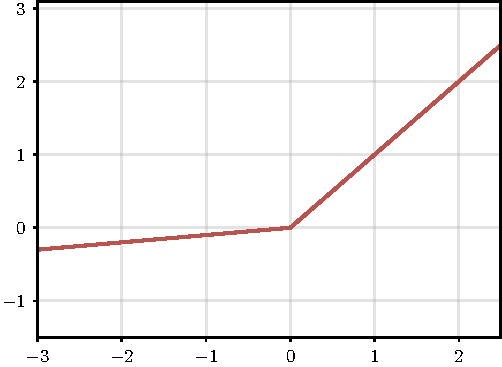
\includegraphics[width=1.0\textwidth]{images/activation_function_LeakyReLU.pdf}
    \caption{LeakyReLU}
    \end{subfigure}
    \hfill
    \begin{subfigure}[b]{0.18\textwidth}
    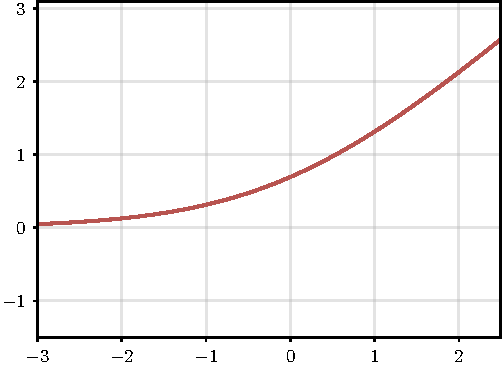
\includegraphics[width=1.0\textwidth]{images/activation_function_Softplus.pdf}
    \caption{Softplus}
    \end{subfigure}
    \hfill
    \begin{subfigure}[b]{0.18\textwidth}
    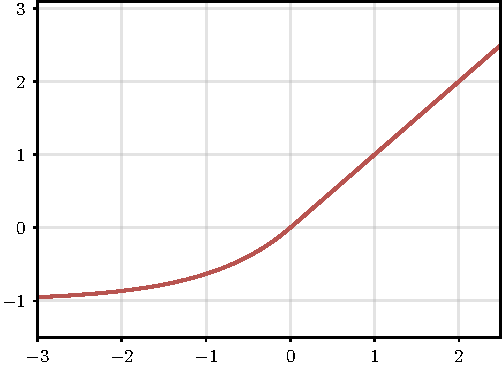
\includegraphics[width=1.0\textwidth]{images/activation_function_ELU.pdf}
    \caption{ELU}
    \end{subfigure}
    \hfill
    \begin{subfigure}[b]{0.18\textwidth}
    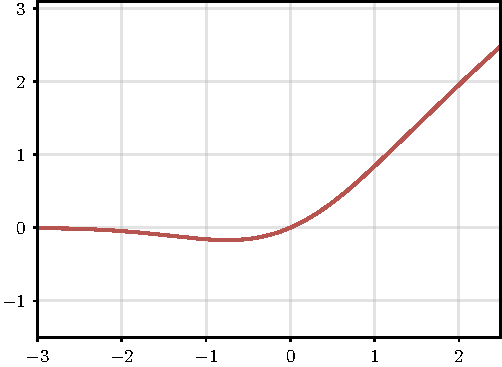
\includegraphics[width=1.0\textwidth]{images/activation_function_GELU.pdf}
    \caption{GELU}
    \end{subfigure}
    \hfill
    \caption{Визуальное сравнение ReLU и четырех вариантов: LeakyReLU \eqref{eq:leaky_relu}, Softplus \eqref{eq:softplus}, ELU \eqref{eq:elu}, и GELU. LeakyReLU показан с $\alpha=0.1$ для лучшей визуализации, но на практике $\alpha$ может быть ближе к $0$ (например, $0.01$)..}
    \label{fig:activation_functions}
\end{figure}

Можно получить несколько обучаемых вариантов каждой функции, добавив к ним обучаемые параметры. Например, распространенный обучаемый вариант Swish с четырьмя параметрами $\left\{a,b,c,d\right\}$ получается как:
%
\begin{equation}
\text{Trainable-Swish}(s)=\sigma(as+b)(cs+d)
\label{eq:trainable_swish}
\end{equation}
%
Мы также можем проектировать \textbf{непараметрические} функции активации, в смысле функций активации, которые не имеют фиксированного числа обучаемых параметров. Например, рассмотрим общий набор (необучаемых) скалярных функций $\phi_i$, индексированных целым числом $i$. Мы можем построить полностью гибкую функцию активации как линейную комбинацию $n$ таких базисов:
%
\begin{equation}
\phi(s) = \sum_{i=1}^n \alpha_i \phi_i(s) \,
\label{eq:non_parametric_af}
\end{equation}
%
где $n$ — гиперпараметр, а коэффициенты $\alpha_i$ обучаются градиентным спуском. Они могут быть одинаковыми для всех функций или разными для каждого слоя и/или нейрона. В зависимости от выбора $\phi_i$ мы получаем разные классы функций: если каждая $\phi_i$ — это ReLU, мы получаем \textbf{адаптивную кусочно-линейную} (APL) функцию \cite{agostinelli2014learning}, а для более общих ядер мы получаем \textbf{ядерную функцию активации} (KAF) \cite{marra2018learning,scardapane2019kafnets}. Еще более общие модели можно получить, рассматривая функции с несколькими входами и несколькими выходами \cite{li2023generalized}. См. \cite{apicella2021survey} для обзора.

В общем, нет ответа на вопрос «какая ФА лучшая», поскольку это зависит от конкретной задачи, набора данных и архитектуры. Помимо своей производительности, ReLU является распространенным выбором также потому, что доступны высокооптимизированные ядра кода, и она добавляет незначительные накладные расходы. Важно учитывать фундаментальный вычислительный компромисс, заключающийся в том, что при заданном бюджете более сложные ФА могут привести к меньшей ширине или меньшей глубине, что потенциально снижает производительность всей архитектуры. По этой причине ФА с большим количеством обучаемых параметров менее распространены.

\begin{supportbox}{Варианты дизайна}
Не каждый слой вписывается в рамки \textit{линейных проекций} и \textit{поэлементных} нелинейностей. Например, \textbf{вентильный линейный блок} (GLU) \cite{dauphin2017language} сочетает структуру \eqref{eq:trainable_swish} с мультипликативными (Адамара) взаимодействиями:
%
\begin{equation}
f(\mathbf{x}) = \sigma\left(\mathbf{W}_1\mathbf{x}\right)\odot\left(\mathbf{W}_2\mathbf{x}\right)
\label{eq:glu}
\end{equation}
%
где $\mathbf{W}_1$ и $\mathbf{W}_2$ обучаются. Другой распространенный вариант, SwiGLU, заменяет сигмоиду в \eqref{eq:glu} на функцию Swish \cite{shazeer2020glu}. В сети \textbf{maxout} \cite{goodfellow2013maxout} каждый блок производит максимум из $k$ (гиперпараметр) различных проекций. Замена линейной проекции $\mathbf{W}$ на матрицу обучаемых нелинейностей $W_{ij} \rightarrow \phi_{ij}(x_j)$ вида \eqref{eq:non_parametric_af} также была предложена недавно под названием \textbf{сети Колмогорова-Арнольда} (KAN, \cite{liu2024kan}).
%
\end{supportbox}

\section*{От теории к практике}

\begin{wrapfigure}{r}{3.0cm}
\vspace{-3em}
\includegraphics[width=3.0cm]{images/shutterstock_2075221579.jpg}
\vspace{-5em}
\end{wrapfigure}

Эта глава ввела два ключевых требования для любого универсального фреймворка для обучения дифференцируемых моделей:

\begin{enumerate}
\item Способ обработки больших наборов данных, которые необходимо перемешивать, разделять на мини-пакеты и перемещать туда и обратно из GPU. В PyTorch большая часть этого реализована через интерфейсы {\mintinline{python}{Dataset}} и \mintinline{python}{DataLoader}, как в Листинге \ref{code:data_loader}.\footnote{\url{https://pytorch.org/tutorials/beginner/basics/data_tutorial.html}}
\end{enumerate}

\begin{enumerate}\addtocounter{enumi}{1}
\item Механизм для построения моделей из комбинации базовых блоков, известных как \textit{слои}. В PyTorch слои реализованы в модуле \mintinline{python}{torch.nn}, и их можно компоновать через интерфейс \mintinline{python}{Sequential} или путем подклассирования класса \mintinline{python}{Module}, как в Листинге \ref{code:fully_connected_layer}.
\end{enumerate}

Я предлагаю вам теперь попробовать воспроизвести одно из многих кратких руководств, доступных в документации PyTorch.\footnote{\url{https://pytorch.org/tutorials/beginner/basics/quickstart_tutorial.html}} Все должно быть достаточно ясно, за исключением механизма вычисления градиентов, представленного в следующей главе. Это также хорошее время для изучения HuggingFace Datasets, который сочетает в себе обширный репозиторий наборов данных с интерфейсом для их обработки и кэширования, который не зависит от фреймворка и поддерживается Apache Arrow.\footnote{\url{https://huggingface.co/docs/datasets/en/quickstart}}

JAX не предоставляет высокоуровневых утилит. Для загрузки данных вы можете использовать любой существующий инструмент, включая загрузчики данных PyTorch и HuggingFace Datasets. Для построения моделей самый простой способ — положиться на внешнюю библиотеку. Поскольку JAX полностью функционален, объектно-ориентированные абстракции, такие как Листинг \ref{code:fully_connected_layer}, невозможны. Мое личное предложение — Equinox \cite{kidger2021equinox}, который предоставляет опыт, подобный классовому, путем объединения базовой структуры данных JAX (\mintinline{python}{pytree}) с вызываемыми узлами.
